\section{Graph Problems}
\index{Graph Problems}

\subsection{Concepts}

\subsubsection{Nodes and Edges}
\index{Nodes} \index{Edges}

Graphs are a construct of two basic concepts: \textbf{nodes} (or vertices, or points) represent some object or position, and \textbf{edges} which represent some direct connection or relation between nodes.

A common example is cities and roads. You have some number of cities represented by nodes, that have roads connecting them represented by edges. We can do some interesting things with a graph of cities and roads, such as finding the distance between two given cities and how many other cities we need to pass along the way (which we will cover in the pathfinding section), or finding the minimum number of roads we need in order to get from any one citity to any other city (which is the concept of spanning trees, also covered later).

\subsubsection{Representations}

There are multiple ways to represent graphs when we talk about actually implementing them in code.

\textbf{Edge lists} \index{Edge Lists} are likely the most simple representation of a graph, in which we have an array store each edge in the graph. Nodes are implicit by their value -- an edge is represented as a pair of integers $a$ and $b$ (possibly with additional information like weight) that defines a connection between the $a$th node and the $b$th node.

\inputcpp{code/graph/core_edge_list.cpp}

Unfortunately, edge lists are relative uncommon and aren't the ideal graph representation for the majority of graph algorithms. This is because one of the most common things we want to do with graph algorithms is operate on edges connected to a specific node. With edge lists, this is $O(n)$ -- we have to traverse through the entire list to find what edges are connected to a specific node. We can optimize this somewhat (sort the edge list so all nodes appear in order in $O(n log n)$, then binary search for a specific node in $O(log n)$, for example) but ultimately we can do better with other graph representations for most use cases.

\textbf{Adjacency lists} \index{Adjacency Lists} are a graph representation in which we have an array of each node, where each node stores its edges. This fixes our issue with edge lists, because now we can index directly into a node and operate directly on all of its incident edges. This can either be as an array of \mintinline{cpp}{Node} objects where each \mintinline{cpp}{Node} contains an edge list, or as an array of edge lists. Even simpler, we can have an array where each index is the start node of the edge, and store a list of end node values:

\inputcpp{code/graph/core_adjacency_list.cpp}

Now, we may notice that we improved our accesses for our start node from $O(n)$ to $O(1)$ by using an array instead of a list, with the index equal to the start node of a given edge. Unfortunately, since adjacency lists still use lists, trying determine whether an edge between a specific start node and a specific end node exists is potentially expensive as well -- we would have to iterate through every edge indicent with the start node to find if that specific end node exists. So you may ask, why not use an array again, so that we have a 2D array where end nodes are our index for the inner array?

As it turns out, this is called an \textbf{adjacency matrix}\index{Adjacency Matrices}. We maintain a 2D array of boolean values, so that we can quickly check whether an edge between $a$ and $b$ exists by checking the value of \mintinline{cpp}{edges[a][b]}.

\inputcpp{code/graph/core_adjacency_matrix.cpp}

Now, is any one of these representations strictly better than the others? Not at all! They all have their strengths and weaknesses, namely:
\begin{itemize}
\item Only adjacency matrices can check if an edge between $a$ and $b$ exists in $O(1)$. Edge lists need to iterate through the entire list to find if that edge exists, while adjacency lists have to iterate through the list of edges incident to $a$.
\item If there are only a couple of edges incident to node $a$, only adjacency lists can iterate through those incident edges quickly. Edge lists don't have easy access to find node $a$ and have to search through the entire list, while adjacency matrices have to look through every value of \mintinline{cpp}{edges[a][0..n]} to find incident edges.
\item If there are only a couple of edges in general and you need to iterate through every edge, only edge lists can iterate through them quickly. Adjacency lists require you to iterate through its whole array of size $n$, and adjacency matrices require you to iterate through its entire 2D array -- to go through $n^2$ different values.
\end{itemize}
To generalize, using a list is good if your graph doesn't have a large amount of edges compared to the number of nodes, and you want to iterate through edges rather than access specific ones. Comparatively, using an array is good if your graph has lots of edges relative to the number of nodes, and/or you don't need to iterate through edges and would prefer the $O(1)$ lookup time.

In practice, edge lists are usually not the preferred method -- there are relatively few algorithms or problems that are best implemented by iterating through every edge in arbitrary order. Adjacency lists and adjacency matrices appear fairly frequently, so it's important to know both of them well.

\subsubsection{Directed and Undirected}
\index{Directed Graphs} \index{Undirected Graphs}

One trait of graphs is whether they're directed or undirected.

In a directed graph, edges are one way -- an edge from $a$ to $b$ can be traversed in that order, but you could not go from $b$ to $a$ using that edge.

In contrast, an undirected graph has edges that go in either direction. The edge $a,b$ also represents an edge $b,a$ in that traversal can be done with either $a$ to $b$ or $b$ to $a$.

Our graph representations that we developed above only supported directed graphs. However, when we add an edge $a,b$, we can also add the edge $b,a$ in order to make our representations be equivalent to undirected graphs.

\subsubsection{Cyclic and Acyclic}
\index{Cycles} \index{Cyclic Graphs} \index{Acyclic Graphs} \index{Circuits}

A \textbf{cycle} is a path where the start and end node are the same, but no other edges are traversed more than once (a path that does repeat a non-start node is called a \textbf{circuit} instead). In plainer terms, without traversing the same edges or any nodes multiple times (except the start node exactly twice), cycles are what you find when you end up at the same node as you started.

We call a graph that contains cycles \textbf{cyclic}. In comparison, a graph with no cycles is \textbf{acyclic}. This is relevant because sometimes algorithms work well on acyclic graphs but not on cyclic ones, or alternatively fundamentally only matter for cyclic graphs (such as cycle finding algorithms).

\subsubsection{Connected and Disconnected}
\index{Connectivity} \index{Connected Graphs} \index{Disconnected Graphs}

Two nodes are considered \textbf{connected} when there exists some path between them. Opposite to this, two nodes are \textbf{disconnected} if there isn't a path between them, and by definition no amount of graph traversing from one node will lead you to the other.

When we're talking about the graph as a whole, a \textbf{connected graph} means that every node is connected to every other node. Likewise, a \textbf{disconnected graph} means that at least one pair of nodes is not connected.

In directed graphs, the concept of just being connected isn't always enough. While there might be enough edges in the graph to fully connect every node, the direction of the edges matters and may mean there isn't a valid path between every node. We have to introduce the concept of a \textbf{strongly connected graph} where every node has a valid path to every other node when abiding by direction of edges as well.

In practice, a strongly connected graph not only needs to be cyclic, there needs to be a circuit that traverses every node (while we haven't described Hamiltonian cycles yet keep in mind that this \textit{is not} a Hamiltonian cycle, because we do allow traversing nodes multiple times here).

An informal proof is relatively simple: in order to be strongly connected, we have to be able to pick an arbitrary node and have a valid path to every other node as well, and if we had chosen a different starting node then we would also have to have a valid path from every other node back to our originally chosen arbitrary node. In other words, for every pair of nodes $a$ and $b$ in the graph, there needs to be a valid path from $a$ to $b$ and from $b$ to $a$, which is a circuit by definition.

The \textbf{transitive closure} \index{Transitive Closure} of a graph is a transformation in which edges are created between any connected nodes. For example, if a graph normally contains the edges $\{0,1\},\{1,2\}$, there is no edge for $\{0,2\}$ despite there being a valid path between them. In the transitive closure, we would create the edge $\{0,2\}$ so that every node has an edge directly to every other node it's connected to.

Often, the transitive closure of a graph will be stored as an adjacency matrix, because it generally results in a large amount of edges (with a lot of redundancy).

\subsubsection{Complete}
\index{Complete Graphs}

A graph is considered \textbf{complete} if every node contains an edge to every other node. As a result, the minimum path length from one node to another is always $1$ in a complete graph.

A complete graph with $n$ nodes will contain $\frac{n(n-1)}{2}$ edges. While often assumptions can be made about complete graphs that simplify problems immensely, the large amount of edges may also make common algorithms expensive and ineffective.

\subsubsection{Weighted}
\index{Edge Weights} \index{Weighted Graphs}

Edges can also have \textbf{weights}.

A graph that does not include weights (or equivalently, one where every edge has a weight of 1) is considered an unweighted graph. A graph with edges that include different weights is considered a weighted graph.

\subsubsection{Grids}
\index{Grids}

Grids are a specific case of graphs, but are extremely common. You are given a (usually 2D) array where. In graph form, each element represents a node, has an edge between each of its neighbors. 

in Euclidean geometry the distance between two points will be the length of the line segment directly connecting them (in other words, $d = \sqrt{(x_2 - x_1)^2 + (y_2 - y_1)^2}$. Often, the concept of \textbf{Manhattan distance} or \textbf{taxicab distance} will be used instead, in which the path cannot be diagonal and must consist of lines going either horizontally or vertically (and as a result, $d = |x_2 - x_1| + |y_2 = y_1|$).

\subsection{Pathfinding}
\index{Pathfinding}

One of the most common tasks with graphs is to find a path between two nodes, or the distance between them. As we will see, traversing the graph in this manner is a common subtask in several other, more complicated graph algorithms as well.

It's important to know that, in general, there isn't any single pathfinding algorithm that you should always use. Each have their own strengths and weaknesses that are only relevant in certain circumstances, or come with specific restrictions that make them only worthwhile on specific types of graphs.

\subsubsection{Depth First Search}
\index{Depth First Search}

Out of all the pathfinding algorithms, the depth first search is the easiest conceptually. Starting at a specific node, we explore a path as long as possible without revisiting the same node twice (until we either find our target end node, or we reach a point where we have no more unvisited neighbors to explore). If we don't find the end node, we try again with a slightly different path -- the last time we had multiple unvisited neighbors to a node (and we ended up going down the first path), let's no try the next neighbor and attempt that path.

{\centering 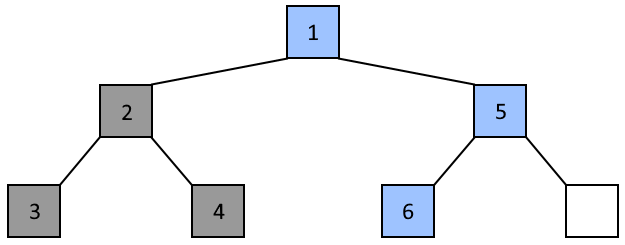
\includegraphics[width=\textwidth]{images/graph/dfs.png}}
\textit{In the above image, blue is the proper path from $1$ to $6$ while grey is explored nodes that are not involved in the proper path.}

In the above example, we start at node $1$ and want to find whether a path exists to node $6$. A DFS will begin by checking $\{1\}$, $\{1, 2\}$, $\{1, 2, 3\}$, $\{1, 2, 4\}$, $\{1, 5\}$, $\{1, 5, 6\}$, and at that point can say there is a path between $1$ and $6$. 

We can model this using a stack data structure, where we add all unvisited neighbors of a node into the stack. If at any point we encounter the end node, we know there's a valid path and can return \mintinline{cpp}{true} then. If our stack is empty, we know we've checked every node connected to our starting position without finding the end node.

\inputcpp{code/graph/dfs_stack.cpp}

A keen eye can notice that using a stack like that is very similar to recursion -- in fact the code for a DFS becomes significantly shorter when we convert it to use recursion instead:

\inputcpp{code/graph/dfs_recursive.cpp}

\subsubsection{Breadth First Search}
\index{Breadth First Search}

Breadth first search is similar to depth first search, except instead of trying to search through the first path possible (prioritizing \textit{depth}) we try to search through every neighbouring node (priorizing \textit{breadth}).

The simplest approach to implementing this is to take our stack-based implementation for DFS and use a queue instead. This means that, instead of trying the most recently added node for the next iteration as we would in a DFS, we will use the oldest node for the next iteration.

\subsubsection{Dijkstra's Algorithm}
\index{Dijkstra's Algorithm}

DFS and BFS, as can be noted, doesn't consider weighted graphs -- if we exit at the first time we encounter the target end node, DFS will give us some valid path and BFS will give us a path with the minimum number of edges. In neither case are these edges necessarily with the minimum total weight (in BFS's case, we may find a solution in one edge with weight of 100, when the minimum total weight would be two edges each with weight 1).

Dijkstra's algorithm is a solution to this. It's also implemented like DFS or BFS except we use a priority queue, where the weight of our current path is how we base the priority (we consider lower weights before higher weights). Additionally, rather than storing whether a node is visited or not, we store the current best (minimum) weight of a path we've found (defaulting to infinity, or some huge number that won't be encountered normally). Using this, when we consider the neighbors of an node, rather than checking if that node is already visited we check if our current node's best weight + the weight of our next edge, and add that to our priority queue if so.

\subsubsection{A* Algorithm}
\index{A* Algorithm}

The A* algorithm can be considered a generalization of Dijkstra's, in which we use a heuristic function to (hopefully) improve performance.

Under Construction

\subsubsection{Bellman-Ford Algorithm}
\index{Bellman-Ford Algorithm}

A restriction with Dijkstra's is that it can't handle negative weights properly -- there are specific cases where a negative weight can break the assumptions that Dijkstra's makes.

The Bellman-Ford algorithm can work with this, both by being able to handle negative weights (when there are no negative cycles) and being able to detect negative cycles (in which case there is no shortest path).

Under Construction

\subsubsection{Floyd-Warshall Algorithm}
\index{Floyd-Warshall Algorithm}

So far the algorithms we've considered have been single-source shortest path algorithms -- namely that we have a specific starting node. What if we want to determine the shortest path distance between any two arbitrary points? We would need an all-pairs shortest path algorithm instead.

Floyd-Warshall meets these requirements. It works with negative weights as well, assuming that there are no negative weight cycles.

Under Construction

\subsubsection{Path Reconstruction}
\index{Path Reconstruction}

For DFS, BFS, Dijkstra's, etc. we can include an auxillary array that represents some data about each node. In order for the algorithms to work, we already include an array that determines whether a node has been visited for DFS and BFS, and for Dijkstra's we include an array that determines the minimum weight of a path we've needed so far.

One of the most common ones is a \textit{parent} array, in which every node stores what node came before it in the path. This is useful for path reconstruction, where we want to determine the path taken to get to the end node.

When we set our node as visited (for DFS and BFS) or the weight required (for Dijkstra's) we also set the parent node. Then, after our algorithm is done, we check the parent of the end node, then its parent, then the parent of that node, and so on until we reach the source node. The path is this list of parents in reverse.

\subsection{Union-Find}
\index{Union-Find} \index{Disjoint-Set} \index{DSU}

Union-Find, which also goes by the name of \textit{disjoint-set}, is a data structure that groups connected nodes together into different subsets through operations called \textbf{union} (which connects two nodes together, akin to creating an edge) and \textbf{find} (which determines which subset a node belongs to). As a result, Union-Find is well suited for any problem in which you have to determine if two different elements belong to the same set -- this sees applications both by itself in many problems, and as an important part of different graph algorithms.

\subsection{Minimum Spanning Trees}
\index{Spanning Trees} \index{Minimum Spanning Trees}

Many graphs have redundant edges -- between nodes $A$ and $B$ there may be several different paths. A spanning tree of a connected graph is one in which we use a subset of edges (whether we think of it as removing redundant edges or building up only the necessary edges depends on the algorithm we use) so that every pair of nodes has exactly one unique path between them.

A minimum spanning tree is a variant of a general spanning tree, where we want to obtain the minimum total weight among all spanning trees. This is not necessarily unique either, as there easily could be multiple possible minimum spanning trees.

\subsubsection{Prim's Algorithm}
\index{Prim's Algorithm}

Under Construction

\subsubsection{Kruskal's Algorithm}
\index{Kruskal's Algorithm}

Under Construction

\subsection{Strongly Connected Components}
\index{Strongly Connected Components}

Earlier in this chapter we defined the concept of strongly connected graphs: directed graphs where every node can reach every other node. \textbf{Strongly connected components} (or SCCs) are subgraphs in a directed graph that are strongly connected. We can decompose a graph into its strongly connected components, where each node of the graph represents a strongly connected component of the original.

This concept sees some use in various problems. For example, if we want to consider whether a path exists between two nodes in a directed graph with many cycles, then it may be useful to check on the graph of strongly connected components instead. Not only can we immediately know two nodes are connected if they belong to the same strongly connected component, but also the graph we need to check connectivity on is significantly smaller when we're only considering strongly connected components.

\subsubsection{Kosaraju's Algorithm}
\index{Kosaraju's Algorithm}

Under Construction

\subsubsection{Tarjan's Algorithm}
\index{Tarjan's Algorithm}

Under Construction

\subsection{Maximum Flow}
\index{Maximum Flow}

Under Construction

\subsection{Bipartite Graphs}
\index{Bipartite Graphs}

Under Construction

\subsubsection{Determining Bipartite Graphs}

Under Construction

\subsubsection{Maximum Bipartite Matching}
\index{Maximum Bipartite Matching}

Under Construction

\subsection{Eulerian Paths}
\index{Eulerian Paths} \index{Eulerian Cycles}

A Eulerian Path is a traversal of a graph in which every edge is visited exactly once. By consequence each node will also be visited one or more times.

Similarly, a Eulerian Cycle is a traversal of a graph that visits every edge exactly once with the added restriction that it's a cycle and has the same start and end node.

It is relatively easy to verify whether or not a Eulerian Path or Cycle exists. The following conditions must be satisfied:
\begin{itemize}
\item The graph must be connected
\item The degree of each node must be even
\end{itemize}

\subsubsection{BEST Algorithm}
\index{BEST Algorithm}

Under Construction

\subsubsection{Hierholzer's Algorithm}
\index{Hierholzer's Algorithm}

Under Construction

\subsection{Hamiltonian Paths}
\index{Hamiltonian Paths} \index{Hamiltonian Cycles}

A Hamiltonian Path is similar to a Eulerian Path except that it deals with nodes rather than edges -- it's a traversal in which each node is visited exactly once, and by consequence each edge is either visited once or not visited at all.

A Hamiltonian Cycle follows the same convention where we add the restriction that the end node of our traversal also has to be our source node.

Unlike Eulerian Paths and Cycles, verifying whether a Hamiltonian Path or Cycle exists or not is an NP-complete problem for the general case. There are special cases however:
\begin{itemize}
\item a complete graph with $n$ nodes has $(n-1)!/2$ different Hamiltonian Cycles.
\item By Dirac's Theorem, a simple graph with at least 3 nodes contains a Hamiltonian Cycle if every node has a degree of at least $\frac{n}{2}$ where $n$ is the number of nodes in the graph.
\item By Ore's Theorem (which generalizes Dirac's Theorem), a simple graph with at least 3 nodes contains a Hamiltonian Cycle if, for every pair of nodes in the graph, the sum of their degrees is at least $n$ where $n$ is the number of nodes in the graph.
\end{itemize}